\documentclass[11pt]{article}
\usepackage[letterpaper,margin=1in]{geometry}
\usepackage[T1]{fontenc}
\usepackage[utf8]{inputenc}
\usepackage{textcomp,lmodern,microtype}
\usepackage{amsmath,amssymb,graphicx,booktabs,array,longtable}
\usepackage[authoryear,round]{natbib}
\usepackage{caption,hyperref,setspace}
% Indent the first paragraph after headings without an additional package.
\makeatletter
\let\@afterindentfalse\@afterindenttrue
\@afterindenttrue
\makeatother
\setstretch{1.12}
\setlength{\parindent}{1.5em}
\setlength{\emergencystretch}{2em}
\hypersetup{colorlinks=true,linkcolor=black,citecolor=black,urlcolor=blue}
\graphicspath{{../figures/}}
\newcommand{\notes}[1]{\par\smallskip{\footnotesize\emph{Notes.} #1}\par}
\title{Unnumbered Books:\\ISBN Coverage and the Measurement of\\Author-Published Books in Portugal}
\author{Shreeniket Bendre}
\date{11 November 2026}
\begin{document}
\maketitle
\begin{abstract}
\indent In 2015, Portugal's ISBN agency recorded a sharp fall in assignments to author-publishers. How much of the apparent decline reflects fewer recorded books, and how much reflects changing ISBN coverage? I examine that question using national-bibliography records around Portugal's reform of ISBN charges and application procedures. Between 2014 and 2015, records provisionally classified as author-published fell from 392 to 343, while their ISBN-bearing subset fell from 240 to 171. Comparing these counts within the same bibliography assigns 60.6\% of the ISBN-bearing series' log decline to lower identifier coverage. Coverage fell from 58.5\% in 2010--14 to 51.3\% in 2015--19; excluding 2014 leaves a 6.3-percentage-point decline. Alternative dates and classification rules preserve its direction. Selective registration can consequently distort measured output growth and producer shares, and can bias empirical estimates when coverage changes with policy or market conditions. Independent human validation remains necessary: asymmetric classification errors can eliminate the pooled decline. The analysis documents a discrepancy in recorded counts, without identifying its cause or publications absent from the bibliography. Reporting ISBN coverage alongside bibliographic counts exposes an observation margin that ISBN-only statistics conceal.
\end{abstract}
\noindent\textbf{Keywords:} ISBN; author-publishing; national bibliography; measurement error; publishing statistics; Portugal.\\
\textbf{JEL codes:} L82, Z11, C81.

\section{Introduction}

In 2015, Portugal appeared to experience a sharp contraction in author-publishing. The country's ISBN agency assigned 617 identifiers to author-publishers, down from 988 the year before: a fall of 37.6\%. Yet the national bibliography tells a different story. The number of records classified as author-published fell from 392 to 343, or 12.5\%. The contrast raises a simple question: how much of a decline in ISBN-based publishing statistics reflects fewer recorded books, and how much reflects fewer identifiers?

Obtaining an ISBN and publishing a book are different events. A book may appear without an ISBN, and an identifier may be assigned before a book ever appears. The agency and bibliography also classify publishers differently. Their headline changes cannot simply be subtracted. But the bibliography contains books both with and without ISBNs, making it possible to compare two counts of the same recorded population.

The main finding comes from that comparison. Among books classified as author-published, ISBN-bearing records fell from 240 to 171, or 28.8\%, while records without an ISBN increased from 152 to 172. An exact decomposition separates the change in the total recorded count from the change in the share carrying an ISBN. Lower coverage accounts for 0.205 of the 0.339 log-point decline in ISBN-bearing records, or 60.6\%. Much of the movement in this indicator therefore comes from the identifier margin rather than the recorded book count.

Portugal's institutional change gives the comparison a clear setting. In January 2015, APEL began charging for the previously subsidized ISBN service and required online applications. Existing publisher prefixes remained valid until exhausted \citep{apel2014,apel2015}. For an individual author requesting a number, the new tariff listed a \texteuro{}15 charge before VAT. An established publisher could still have unused numbers. Because charges and application procedures changed together, their separate effects cannot be identified here.

The coverage decline is not confined to the unusually high 2014 baseline. Across 2010--14 and 2015--19, ISBN coverage among classified author-published books fell by 7.2 percentage points. Excluding 2014 leaves a 6.3-point decline. Coverage among other bibliography records fell by 0.6 points over the full windows. Both comparisons measure the share of recorded books carrying an ISBN, the same outcome used in the decomposition.

Existing studies describe the difficulty of defining and recording non-traditional books, the bibliographic obstacles facing self-published work, and libraries' selective collection of it \citep{bradley2011,holley2014,dilevko2006}. This paper measures how ISBN coverage changes within a national bibliography and shows what that change does to an output indicator. A shared catalogue denominator makes the discrepancy observable; the longer comparisons establish how much its size depends on the chosen baseline.

If authors publish the same books but register fewer of them, an ISBN-based statistic will suggest that publishing has shrunk. If smaller producers are more likely to stop registering, the remaining records will also make larger publishers appear more prominent. A researcher studying a policy change could then mistake a change in who gets counted for a change in economic activity. When coverage varies with the policy or market condition being studied, this becomes nonclassical measurement error: the recording error is related to the explanatory variable. The Portuguese comparison measures one part of that problem directly. Section~\ref{sec:economic} develops its implications for growth, producer shares, and empirical estimates.

Two limits define the evidence. The bibliography cannot reveal books it never captured, and the author-publisher classification still needs independent human validation. The latter matters quantitatively: in one adverse scenario, reclassifying approximately 0.515\% of post-2015 ISBN-bearing negative records as author-published eliminates the pooled coverage decline. I report that sensitivity alongside the main finding and provide a weighted validation design. The claim is about a measurable divergence in recorded counts, not a national production census or a causal estimate of the fee.

\section{Institutional setting and related research}

\subsection{Registration, deposit, and cataloguing}

An ISBN identifies a publication's edition and product form. A different format normally requires a separate number; it does not identify an abstract work or certify its quality. The system facilitates transactions and metadata exchange \citep{isbnagency}. A registration count consequently has a different unit and timing from a count of works produced, sold, deposited, or catalogued.

Three institutional records appear in the Portuguese evidence. Agency assignments record ISBNs allocated to applicants. Legal-deposit registrations record an administrative step associated with printing. National-bibliography records describe catalogued publications, including books without ISBNs. The BNP describes the national bibliography as a record of Portuguese publications received through legal deposit \citep{bnpservice}. Nevertheless, incomplete deposit, cataloguing decisions, metadata omissions, and different processing lags can affect the observed bibliography. The presence of a legal-deposit number does not itself establish receipt, complete coverage, or the date on which a book became available.

An author approaching APEL at the end of 2014 encountered a service whose public subsidy was about to end. In a letter dated 11 December, APEL announced charges from 1 January 2015. A non-professional applicant seeking an individual author-edition ISBN would face a listed charge of \texteuro{}15 before VAT. Larger applicants faced block tariffs, while association members faced an increase in their subscription. The letter also listed a \texteuro{}25 initial-system registration charge for a first prefix requested by a non-member; its wording does not establish that every individual author-edition request incurred that additional charge \citep{apel2014}.

Payment was only part of the change. Requests moved to an exclusively online form, as a contemporaneous APEL webpage confirms \citep{apel2015}. At the same time, previously assigned publisher prefixes remained valid until exhausted. An established publisher with unused numbers could continue issuing books from that allocation, while an applicant needing a new number faced the revised service. The reform therefore changed the conditions of registration unevenly. The preserved documents establish those rules; applicants' actual costs and remaining allocations are not observed.

\subsection{What the study adds}

\citet{bradley2011} describe the heterogeneous expansion of non-traditional publishing and the difficulty of interpreting conventional output measures. \citet{bradley2012} study a sample of books from fee-based publishing services, providing an empirical account of that segment's publications and metadata. Those services are distinct from the personal author-publisher names used here. Their work underscores why a definition of self-publishing must accompany any count.

\citet{dilevko2006} examine library collection of titles from self-publishing houses. \citet{holley2014} considers the challenge self-publishing poses for universal bibliographic control. These studies concern which books enter the systems used to describe and discover publications. The present study examines a second selection margin: ISBN presence among books that have already entered a national bibliography. It cannot estimate the first margin, entry into that bibliography, from the catalogue alone.

The broader measurement literature similarly shows that interpreting a social or economic quantity through a single institutional source can be misleading. For example, \citet{meyer2019} show that linked survey and administrative records materially change estimates of income and programme coverage. \citet{bhandari2020} document economically relevant differences in business-income, valuation, and return measures across survey and other data sources, including problems of sample representativeness. The Portuguese records here are not a linked census of all publication and registration events. Their value is instead a shared within-bibliography denominator on which one component of selective observation can be measured.

The Portuguese case shows how the meaning of a publishing statistic can change over time. Counting identifiers measures recorded publishing activity reliably only to the extent that the relationship between books and identifiers is understood. Here, that relationship can be examined directly for books already in the bibliography.

\section{Data, definitions, and validation}

\subsection{Bibliography population and classification}

The analysis joins membership in BNP's national-bibliography dataset to the fuller catalogue metadata by bibliographic record identifier. The bibliography and catalogue are separate BNP datasets distributed through the Portuguese public-data portal (\citealp{bnpdata}; \citealp{bnpcatalogue}). The project identifies the national-bibliography extraction as the January 2026 snapshot. The replication documentation separates that source snapshot from this revision's frozen analytical export.

The previous draft's larger extraction comprised 313,379 records labelled as books in the bibliography export, before matching full metadata or applying this paper's date, print, and country restrictions. Of those, 305,303 match the full catalogue by record identifier; 8,076 do not. Among matched records, 502 lack a usable publication year and 39,579 fall outside 2005--25, leaving 265,222. Publication year is parsed from the publication statement, with a coded-field fallback. Excluding 212 records that fail the print-monograph filter and then 2,235 without Portuguese country metadata leaves 262,775 unique records. These are exclusions from the analytical population, not estimates of books that disappeared after the reform. Appendix~\ref{app:population} reports the complete count reconciliation, including unmatched records whose eligibility cannot be established.

The principal analysis ends in 2019: there are 189,663 retained records in 2005--19 and 130,324 in the main 2010--19 window. Later records are retained in the export only so that alternative legal-deposit dating can include a record whose publication year falls outside the main window. No post-2019 substantive comparison enters the headline estimates. The prior 313,379-record figure and the revised 262,775-record figure therefore describe different stages of the same extraction, not conflicting estimates of one population.

A record carries an ISBN when the existing parser identifies at least one valid ISBN for a print manifestation. The count is one bibliographic record, regardless of how many ISBNs are attached to it. ``Without ISBN'' therefore means no qualifying ISBN was parsed from the metadata. It does not establish that the physical book never had an ISBN. Differences in how identifiers are recorded are part of the measurement problem.

The primary author-published flag combines normalized personal author--publisher name matching with explicit author-edition language. Portuguese name variants, initials, and particles are handled by the existing classifier; the same rule is used across years. A second, earlier rule provides a sensitivity check. The operational class excludes many books published under a separate press or service imprint and is not equivalent to all independent publishing. Nor is it equivalent to APEL's author-edition prefix or CERLALC's agency-defined author-publisher category. I use ``classified author-published'' to refer to this record-based definition.

\subsection{The estimand and its limits}

Let $C_t$ be all records classified as author-published in the observed bibliography for publication year $t$, and $I_t$ the subset with a parsed ISBN. Define coverage as $p_t=I_t/C_t$. For any two years,
\begin{equation}\label{eq:identity}
\Delta\log I_t=\Delta\log C_t+\Delta\log p_t.
\end{equation}
The identity separates changes in the classified record count from changes in ISBN coverage. It requires a common record population for numerator and denominator. It cannot be applied by subtracting APEL's author-publisher registrations from total monograph deposit registrations.

Even with a perfectly classified catalogue, $C_t$ need not equal author-published output. If $T_t$ denotes all eligible publications and $c_t=C_t/T_t$ denotes their capture in the bibliography, then $\Delta\log I_t=\Delta\log T_t+\Delta\log c_t+\Delta\log p_t$. Only the sum of the first two terms is observed here. Moreover, $p_t$ is coverage conditional on bibliographic capture, not the ISBN rate among all published books. Recovering that population rate would require additional data or untested assumptions about how capture depends on ISBN status.

For longer windows, coverage is calculated from pooled record counts. An equal-year-weighted calculation is reported separately. The comparison with other records is
\begin{equation}\label{eq:comparison}
D=(p_{A,post}-p_{A,pre})-(p_{O,post}-p_{O,pre}),
\end{equation}
where $A$ denotes classified author-published records and $O$ all other records. This is a descriptive differential change. Interpreting it as a reform effect would require stable classification and capture, a credible counterfactual trend, and exclusion of simultaneous differential changes.

\subsection{Validation status}

Independent classification validation has not been completed and remains the main requirement before journal submission. Earlier AI assessments of catalogue metadata are not human reference labels and do not establish accuracy. Accordingly, precision, recall, and disagreement rates are unreported rather than inferred from those assessments. The sensitivity exercise identifies errors worth investigating; it cannot establish how often those errors occur. Independent coding and adjudication must therefore precede claims that the classification-based findings have been validated.

The prepared validation design samples records within publication year $\times$ predicted class $\times$ ISBN status. An initial 800-record sheet allocates 20 records to each of 40 cells. A precision-oriented extension expands the same design to 2,000 records: 20 per predicted-positive cell, 120 per ISBN-bearing predicted-negative cell, and 40 per non-ISBN predicted-negative cell. The larger allocation to negative records addresses low class prevalence. Pilot and full sheets overlap by design and must not be treated as independent samples.

Coders receive bibliographic evidence while predicted flags, ISBN fields, years, and sampling weights are withheld. Metadata alone validates a metadata-defined construct. Adjudicating actual publishing arrangements requires additional evidence from the book or publisher. Ambiguous cases must be retained and resolved or bounded. Appendix~\ref{app:validation} specifies weighting and reporting. All present findings remain conditional on the existing machine labels.

\section{Main results}

\subsection{The 2014--15 discrepancy}

\begin{table}[htbp]\centering\small
\caption{Agency assignments and national-bibliography records}\label{tab:counts}
\begin{tabular}{lrrr}\toprule
Series & 2013 & 2014 & 2015\\\midrule
Agency assignments to author-publishers & 718 & 988 & 617\\
All classified author-published records & 313 & 392 & 343\\
With an ISBN & 185 & 240 & 171\\
Without an ISBN & 128 & 152 & 172\\
ISBN coverage (\%) & 59.1 & 61.2 & 49.9\\
\bottomrule\end{tabular}
\notes{Agency figures are CERLALC author-publisher assignments. Remaining rows use one BNP-derived record population and the provisional author-publisher classifier. The agency and bibliography populations differ; their levels are not directly subtractable.}
\end{table}


Table~\ref{tab:counts} distinguishes the agency series from the within-bibliography counts. Agency assignments to author-publishers fell from 988 to 617, whereas classified bibliography records fell from 392 to 343. Differences in agency categories, assignment timing, catalogue capture, and units prevent interpreting the gap between those percentage changes as missing books. The within-bibliography comparison avoids that subtraction.

ISBN coverage among classified author-published records fell from 61.2\% in 2014 to 49.9\% in 2015, a decline of 11.4 percentage points. The corresponding 95\% Wilson intervals are 56.3--65.9\% and 44.6--55.1\%. These are conditional binomial reference intervals for the recorded class. The underlying counts enumerate the retained snapshot; the intervals do not quantify errors in classification, bibliography coverage, or the national reform's effect.

\begin{figure}[htbp]\centering
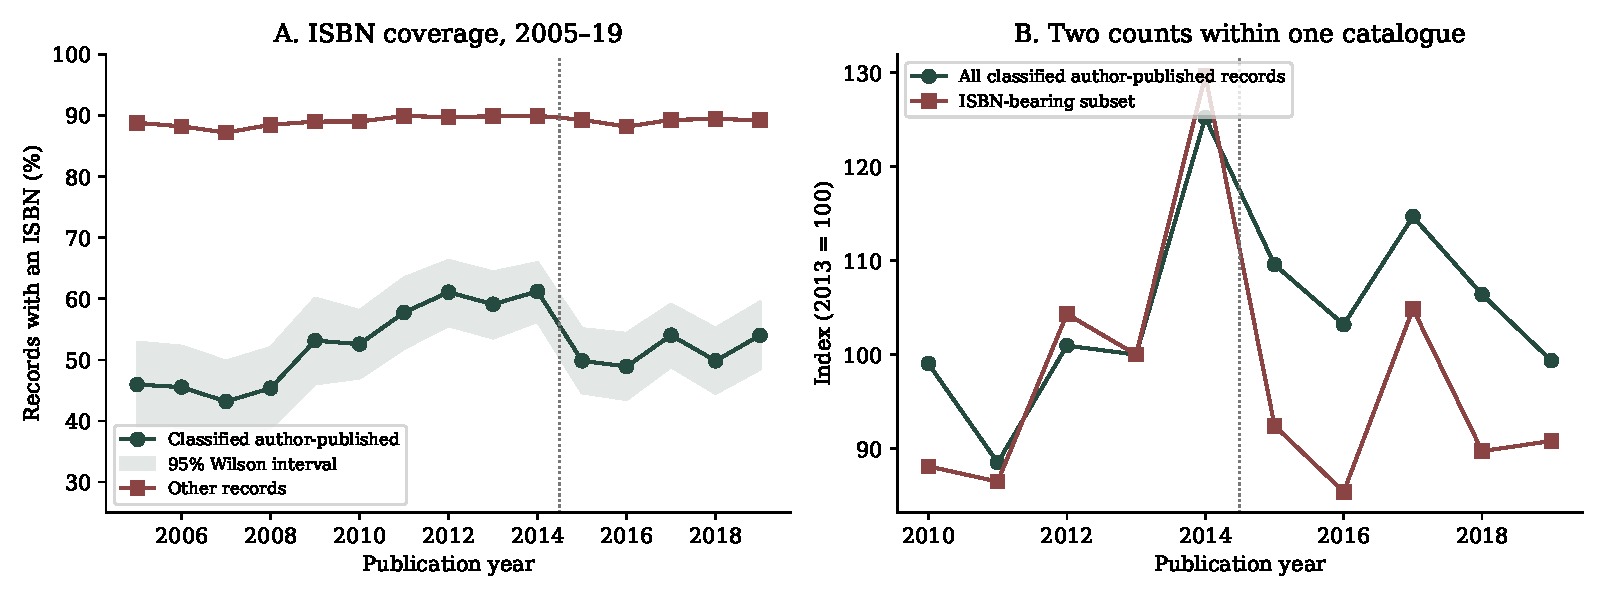
\includegraphics[width=\linewidth]{figure1_trends.pdf}
\caption{ISBN coverage and recorded author-published books in Portugal}\label{fig:trends}
\notes{Panel A shows ISBN presence among classified author-published and other records. Shading is the conditional 95\% Wilson interval for the former. Panel B indexes two counts from the same classified catalogue population to 2013. The vertical line separates 2014 and 2015. Source: frozen BNP-derived analytical records.}
\end{figure}

Applying Equation~\ref{eq:identity} gives
\begin{equation}\label{eq:headline}
\underbrace{\log(171/240)}_{-0.339}
=\underbrace{\log(343/392)}_{-0.134}
+\underbrace{\log[(171/343)/(240/392)]}_{-0.205}.
\end{equation}
The coverage term is 60.6\% of the ISBN-bearing series' log decline. At the 2014 coverage rate, 343 classified records would contain 210 ISBN-bearing records, compared with 171 observed. Holding the coverage rate fixed therefore produces a difference of 39 records. This is an accounting reference, not a count of ISBN purchases deterred by the reform.

\begin{figure}[htbp]\centering
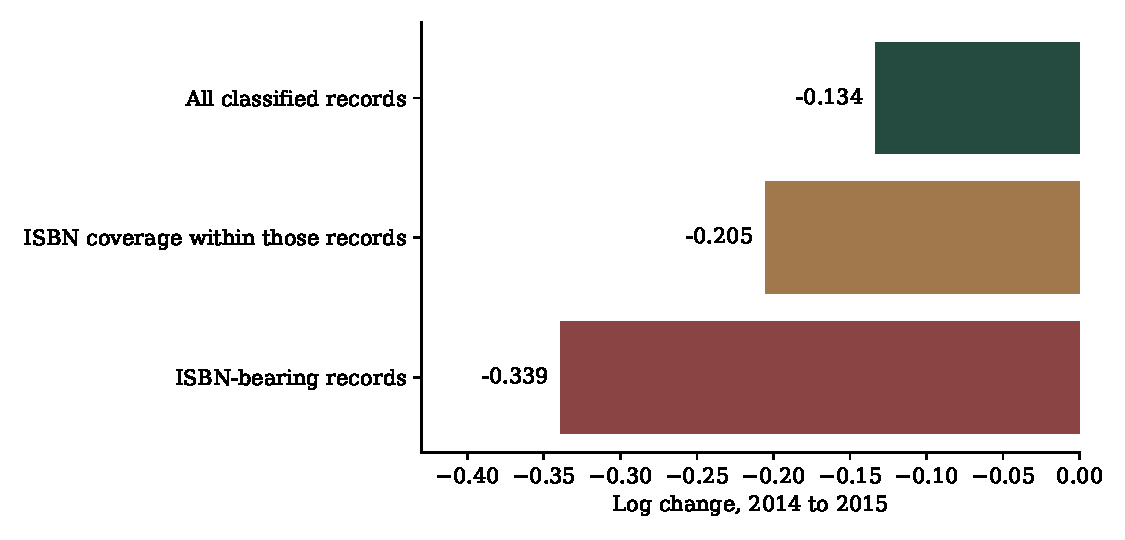
\includegraphics[width=.88\linewidth]{figure2_decomposition.pdf}
\caption{Decomposing the decline in ISBN-bearing author-published records}\label{fig:decomp}
\notes{The first two bars sum to the third. All terms use the same bibliography population and the same classification rule. The 60.6\% coverage fraction is specific to 2014--15. No causal attribution is involved.}
\end{figure}

The baseline matters. In 2013, the bibliography contained 313 classified author-published records, including 185 with ISBNs. Relative to that year, 2015 has 9.6\% more classified records but 7.6\% fewer ISBN-bearing records. Coverage falls from 59.1\% to 49.9\%. In log terms, a positive record-count component offsets part of a negative coverage component, so the coverage contribution exceeds 100\% of the net ISBN-bearing decline. This is valid accounting, but it makes a single ``percentage explained'' unsuitable as a general structural parameter.

\subsection{The longer-run comparison}

In 2010--14, 941 of 1,608 classified author-published records carry ISBNs, a rate of 58.5\%. In 2015--19, the corresponding count is 857 of 1,669, or 51.3\%. The pooled decline is 7.2 percentage points. Average annual classified counts increase slightly, from 321.6 to 333.8, while average annual ISBN-bearing counts fall from 188.2 to 171.4. Thus, the longer-window evidence does not support describing the episode simply as a contraction in recorded author-published output.

Other books have much higher ISBN coverage: 89.7\% in the pre-period and 89.1\% afterward. Their 0.6-point decline yields a 6.5-point differential decline for the author-published class. The groups differ in scale, publishing arrangements, prior trends, and exposure to unused ISBN blocks. Their comparison controls arithmetically for a common change in the rest of the observed catalogue; it does not establish a causal counterfactual.

The annual series also shows why 2015 should not be treated as the beginning of an indefinitely widening gap. ISBN coverage among classified author-published books is 48.9\% in 2016, 54.0\% in 2017, 49.8\% in 2018, and 54.0\% in 2019. Pre-2015 coverage itself had risen from lower levels in the mid-2000s. The evidence is a reversal relative to the immediate pre-reform period, not a monotone decline across the entire observed history.

\section{Robustness and interpretation}

\subsection{Alternative windows and definitions}

\begin{table}[htbp]\centering\small
\caption{ISBN coverage under alternative comparisons}\label{tab:robust}
\begin{tabular}{p{.41\linewidth}rrrr}\toprule
Specification & Pre (\%) & Post (\%) & Change (pp) & Diff. (pp)\\\midrule
Pooled 2010--14 vs 2015--19 & 58.5 & 51.3 & -7.2 & -6.5\\
Exclude 2014 & 57.6 & 51.3 & -6.3 & -5.8\\
Equal weight to each year & 58.3 & 51.3 & -7.0 & -6.4\\
Original classification rule & 58.3 & 50.3 & -8.0 & -7.4\\
Exclude unidentified publishers & 58.5 & 51.3 & -7.2 & -6.9\\
Exclude government publications & 58.5 & 51.3 & -7.1 & -6.6\\
Legal-deposit-number year & 59.4 & 51.6 & -7.8 & -7.2\\
Catalogue entry dated by 2020 & 58.6 & 51.0 & -7.5 & -7.1\\
\bottomrule\end{tabular}
\notes{Pre: 2010--14; post: 2015--19, with the indicated exclusions or dating changes. Diff. is the coverage change relative to other records, not a causal estimate. Equal-year weights differ from the record-weighted main comparison. Legal-deposit dating uses all records with a parseable deposit year and therefore changes inclusion.}
\end{table}


Excluding 2014 reduces the pre-period coverage rate to 57.6\%. The post-period rate remains 51.3\%, leaving a 6.3-point decline and a 5.8-point differential decline relative to other records. Giving every year equal weight yields a 7.0-point coverage decline. The earlier classification rule produces an 8.0-point decline. Excluding records with unidentified publishers or government flags leaves the direction unchanged (Table~\ref{tab:robust}). These are related uses of the same catalogue and should not be counted as independent replications.

Dating by the year embedded in a parseable legal-deposit number yields a 7.8-point coverage decline and a 7.2-point differential decline. A deposit number records an administrative clock, rather than a verified publication date. Its use also changes the included records: missing or unparseable numbers are excluded, and publication-year boundaries no longer define inclusion. The check demonstrates that the pattern is not unique to the publication-year field. It does not independently validate the reform's timing.

Restricting the main publication-year comparison to records whose catalogue entry year is dated by 2020 yields a 7.5-point decline. This removes some late-entering records from the current snapshot. It cannot reconstruct what the catalogue actually contained in 2020, because entries and fields may have been revised later. A historical sequence of complete snapshots would be needed to assess retrospective revisions directly.

\subsection{Direct forecasts as sensitivity exercises}

I use two direct-outcome forecasts as sensitivity exercises for the assumed continuation of pre-2015 coverage. They do not identify causal effects of the reform. Let $z_t=\log[p_t/(1-p_t)]$. One model sets future $z_t$ to the mean of the most recent five training years. The other fits $z_t=\alpha+\beta(t-2005)+u_t$ to all training years and extrapolates the line, then transforms predictions back to coverage rates. Both describe how much the comparison changes under a flat versus continuing-trend benchmark.

Both models are first trained using only 2005--11 and evaluated on the held-out years 2012--14. Coverage-rate RMSE is 10.1 percentage points for the five-year mean and 2.1 points for the logit trend. Refitting with data through 2014, the trend predicts coverage rising from 64.2\% in 2015 to 71.8\% in 2019. Observed coverage averages 16.8 points below those predictions. The five-year-mean prediction is 58.4\%; the observed post-period average is 7.0 points lower.

\begin{figure}[htbp]\centering
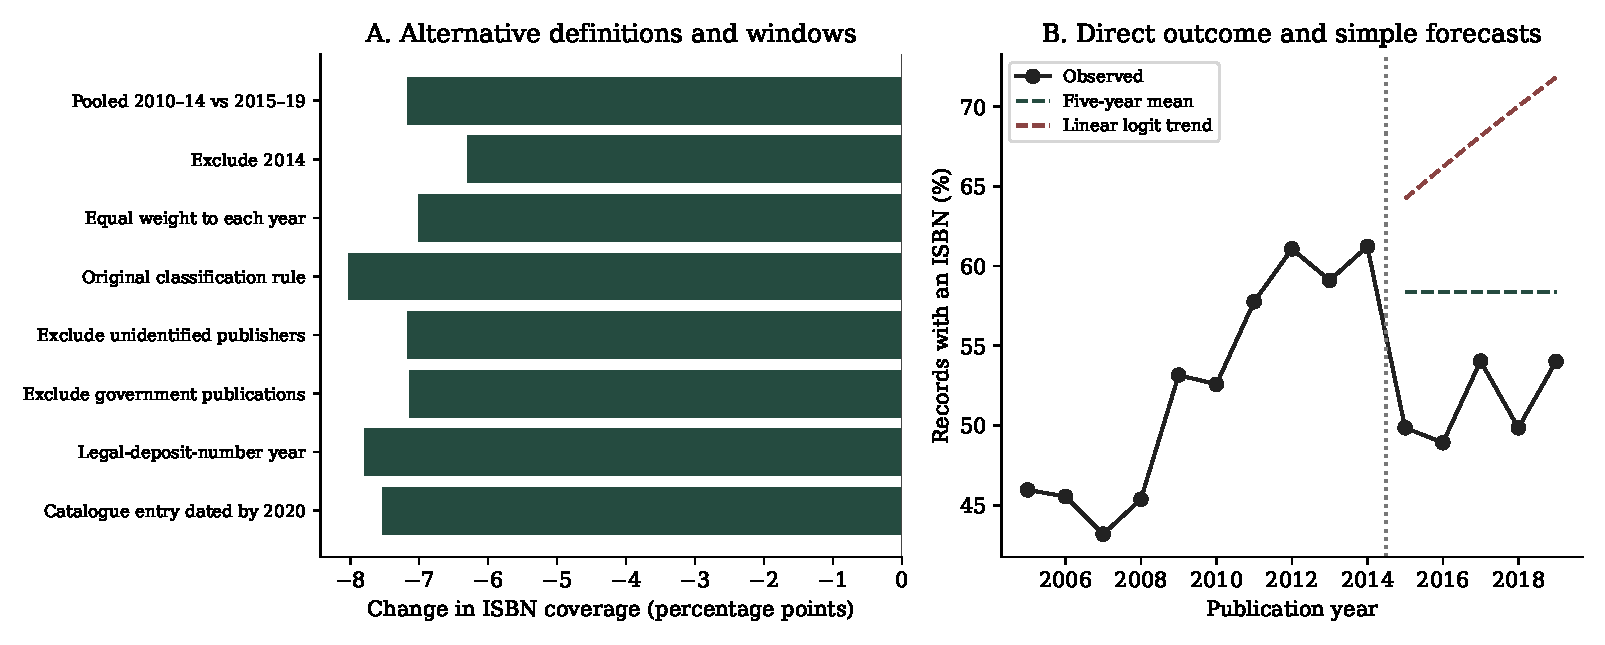
\includegraphics[width=\linewidth]{figure3_robustness.pdf}
\caption{Sensitivity of the direct ISBN-coverage outcome}\label{fig:robust}
\notes{Panel A shows post-minus-pre coverage changes using Table~\ref{tab:robust}'s definitions. Panel B compares observed coverage with two forecasts fit through 2014. Holdout comparison uses 2005--11 training and 2012--14 evaluation. Forecast differences are assumption sensitivity, not a confidence band or a range of causal effects.}
\end{figure}

The difference between these forecasts shows how strongly the apparent departure depends on the assumed trajectory. The trend fits the single three-year holdout better, but its rise need not continue for another five years. These are sensitivity exercises, not causal counterfactuals or confidence limits: they leave national shocks, classification error, and catalogue selection unresolved. The accounting result does not depend on either extrapolation.

\subsection{Classification errors capable of changing the result}

Uniform label error is an inadequate stress test. If precision is identical among ISBN-bearing and non-ISBN predicted positives, removing false positives in the same proportion leaves coverage unchanged. ISBN-specific and period-specific errors can change it substantially.

For period $s$ and ISBN status $h$, let $A_{sh}$ be the predicted-positive count and $O_{sh}$ the predicted-negative count. Define $\pi_{sh}=P(\text{true author-published}\mid\text{predicted positive},s,h)$ and $q_{sh}=P(\text{true author-published}\mid\text{predicted negative},s,h)$. The latter is an omission probability among negative records, not the conventional false-negative rate. Assumed corrected counts are
\begin{equation}\label{eq:correction}
\widetilde C_{sh}=\pi_{sh}A_{sh}+q_{sh}O_{sh},\qquad
\widetilde p_s=\frac{\widetilde C_{s1}}{\widetilde C_{s1}+\widetilde C_{s0}}.
\end{equation}
These expressions quantify assumptions; no error parameters have yet been estimated from independent human labels.

\begin{table}[htbp]\centering\small
\caption{Assumed classification errors and pooled ISBN coverage}\label{tab:sensitivity}
\begin{tabular}{p{.56\linewidth}rrr}\toprule
Scenario & Pre (\%) & Post (\%) & Change (pp)\\\midrule
Uncorrected & 58.5 & 51.3 & -7.2\\
95\% precision, no omissions (uniform) & 58.5 & 51.3 & -7.2\\
90\% precision, 0.1\% omissions (uniform) & 59.8 & 52.9 & -7.0\\
90\% precision, 0.5\% omissions (uniform) & 64.2 & 57.9 & -6.3\\
Post ISBN negatives: 0.1\% omissions only & 58.5 & 52.9 & -5.6\\
Post ISBN negatives: 0.5\% omissions only & 58.5 & 58.3 & -0.2\\
Post no-ISBN positives: 80\% precision only & 58.5 & 56.9 & -1.6\\
\bottomrule\end{tabular}
\notes{Illustrative assumptions, not estimated accuracy or confidence bounds. ``Uniform'' applies the stated precision and negative-record omission probabilities across periods and ISBN groups. In ``only'' rows, all other labels are assumed correct. Omission is the probability of a true author-published record among predicted negatives.}
\end{table}


Table~\ref{tab:sensitivity} illustrates both stability and vulnerability. Assuming 90\% precision and a 0.5\% omission probability uniformly across periods and ISBN groups leaves a 6.3-point decline. In contrast, a 0.5\% omission probability solely among post-period ISBN-bearing predicted negatives nearly eliminates it. There are 56,037 such negative records. Reclassifying about 289 of them, approximately 0.515\%, would raise post-period coverage to the uncorrected pre-period rate. This scenario assumes all other cells are error-free; it is an adverse threshold, not evidence that those errors occurred. A 20\% false-positive share solely among post-period non-ISBN predicted positives leaves a decline of 1.6 points.

The imbalance between class sizes makes this sensitivity consequential. A balanced pilot can check obvious mistakes but may lack power to bound the omissions that matter. For a simple random sample of 100 negative ISBN records, zero observed omissions gives a one-sided binomial 95\% upper limit of about 3\%. At 600 records it is about 0.5\%. These calculations motivate the expanded validation sample, with stratified population weighting still required. They do not guarantee that validation will confirm the result.

\subsection{Why the evidence does not identify a fee mechanism}

The reform combined charges with an online procedure, exposure depended on existing allocations, and the bibliography may select different books in different years. The agency and library categories also differ. Consequently, the decomposition cannot be converted into a price elasticity or a count of authors deterred from registering.

Previously computed same-author results reinforce this caution. Among authors observed before and after the reform, the estimated differential change in ISBN absence is about $-1.0$ percentage point, with an interval spanning $-4.9$ to $2.9$ points. This check does not show the predicted within-author increase. It uses a selected continuing-author sample and cannot rule out changes among entrants, but it weakens an explanation relying entirely on the same authors dropping identifiers.

\section{Economic implications of selective registration}\label{sec:economic}

\subsection{Output growth and producer composition}

Selective registration can make an economic indicator respond to the cost or benefit of being counted. An identifier's usefulness may differ across distribution channels, expected sales, and publishers' existing allocations. If registration entails a fixed expense or administrative task, its burden relative to expected receipts can differ across producers. An observed change in registration may therefore reflect changes in participation as well as production. These are potential selection mechanisms; the present data do not establish their importance or identify which producers responded to the Portuguese reform.

For growth measurement, the relevant distinction follows directly from Equation~\ref{eq:identity}. Growth in ISBN-bearing records equals growth in classified catalogue records plus growth in ISBN coverage. If the broader target is national production, catalogue-capture growth enters as an additional term. Between 2014 and 2015, treating the ISBN-bearing series as catalogue-output growth would add a negative coverage component of 0.205 log points. This is economically consequential for an indicator of product supply even though its monetary or welfare value is unknown. It could lead a researcher to describe reduced observation as reduced production.

Coverage also affects apparent producer shares. Let $s_t=C_{A,t}/(C_{A,t}+C_{O,t})$ be the author-published share of all retained catalogue records, and let $q_t$ be the corresponding share among ISBN-bearing records. Then
\begin{equation}\label{eq:shares}
\frac{q_t}{1-q_t}=\frac{p_{A,t}}{p_{O,t}}\frac{s_t}{1-s_t},
\qquad
\operatorname{logit}(q_t)=\operatorname{logit}(s_t)+\log\frac{p_{A,t}}{p_{O,t}}.
\end{equation}
Thus, changing relative coverage can move the measured author-publisher share even if the composition of catalogue output is unchanged. An ISBN-only decline in that share is not sufficient evidence of displacement by larger publishers. Likewise, product-count concentration or diversity measures can change when some producers' books become less observable. These are statements about counts within the retained catalogue; market shares measured by sales or revenues need not move in the same direction.

Portugal illustrates the size of this distinction. In 2014, classified author-published books account for 392 of 14,496 catalogue records, or 2.70\%, but only 240 of 12,930 ISBN-bearing records, or 1.86\%. In 2015, their catalogue share falls to 343 of 14,953, or 2.29\%, while their ISBN-only share falls to 171 of 13,220, or 1.29\%. Both composition and relative coverage changed. To isolate the coverage margin arithmetically, hold the 2014 catalogue share fixed at 2.70\% and insert the 2015 coverage rates into Equation~\ref{eq:shares}: $p_A=171/343$ and $p_O=13{,}049/14{,}610$. The implied ISBN-only share is 1.53\%. Changing coverage alone can therefore lower that share from 1.86\% to 1.53\% at a fixed catalogue composition. This fixed-composition reference is accounting, not an estimate of the reform's effect.

\subsection{Implications for empirical estimates}

The problem need not have the classical attenuation form associated with a noisy regressor. Suppose a researcher models log publication output as $y_t=\alpha+\beta x_t+u_t$, where $x_t$ measures a policy or market condition. An ISBN-based outcome is $y_t^{obs}=y_t+m_t$, where $m_t=\log c_t+\log p_t$ includes capture and conditional coverage. In a simple regression with an intercept, if $\operatorname{Cov}(x_t,u_t)=0$, the population slope using the observed outcome is
\begin{equation}\label{eq:regression}
\beta^{obs}=\beta+\frac{\operatorname{Cov}(x_t,m_t)}{\operatorname{Var}(x_t)}.
\end{equation}
Measurement error in the outcome affects the slope when selection into the recording system covaries with the explanatory variable. Its direction is unrestricted. If a policy changes registration as well as publishing, the measured response combines both. Additional record-level observations do not remove that common coverage change. Equation~\ref{eq:regression} is a measurement identity under the stated regression assumption, not an estimate of a Portuguese structural relationship.

The same issue arises in empirical studies of entry and product variety. A first observed ISBN may reflect a producer entering the registry, entering a different distribution channel, or issuing a new format, rather than beginning to publish. An apparent exit may reflect non-registration or missing metadata. Registry histories alone do not distinguish those transitions. If entry costs or digital distribution also affect registration incentives, relying on those histories can misattribute a change in visibility to a change in entrepreneurial activity. This paper supplies evidence that the visibility margin varies in the Portuguese catalogue, not a measure of entry, exit, or platform migration.

Selected title counts can also distort ratios when numerator and denominator cover different populations. For example, if a revenue numerator covers a broader set of books than an ISBN-based title denominator, falling registration can mechanically raise measured revenue per title. The present dataset contains neither aligned revenues nor publisher inputs, so it cannot estimate sales productivity or its bias. Similarly, a lower observed variety count does not by itself identify a welfare loss: that requires information about availability, demand, and substitution. The economic contribution is to identify and quantify an observation margin that such applications must address.

\subsection{Reporting and research design}

Before interpreting a fall in a publishing series, a researcher needs to know what was counted. Agency assignments, distinct ISBNs, and bibliography records carrying ISBNs each describe a different event or unit. A useful statistical table should identify that unit and state its category definition, edition and format coverage, timing convention, and treatment of platform or foreign identifiers.

Where an ISBN-independent bibliography exists, reporting its total classified count together with ISBN coverage reveals a selection margin that an ISBN-only indicator conceals. In Portugal, using the 2014--15 ISBN-bearing record decline as a direct estimate of the decline in classified catalogue output would overstate that decline: 28.8\% versus 12.5\%. This comparison is valid within the retained catalogue and classification. It does not certify the smaller number as the national production change.

This distinction matters for regional comparisons as well. CERLALC builds its regional account of publishing from ISBN registration data \citep{cerlalc2020}. Comparing those counts across countries or years requires attention to the systems through which books become visible. Portugal offers a reason to check that relationship, not a correction factor to apply elsewhere.

The immediate research task is to connect the records that already exist: registration, cataloguing, and, where available, independent evidence of publication. Reporting coverage and validating publisher classifications can then separate changes in recording from changes in recorded output. Estimating sales, productivity, or welfare consequences would require further outcomes, but it should begin with a clear account of which books enter the data.

\section{Conclusion}

Within Portugal's national bibliography, ISBN-bearing records and all records provisionally classified as author-published moved apart around 2015. In the 2014--15 comparison, lower ISBN coverage accounts for 60.6\% of the ISBN-bearing series' log decline. The longer-period coverage decline persists when 2014 is excluded and under alternative observed definitions and dates. Its size depends on the comparison, classification accuracy remains unestablished, and plausible asymmetric errors can remove the pooled difference.

The economic lesson is that selective registration can make measured production and producer composition respond to changes in observation. When coverage covaries with a policy or market variable, it can bias empirical estimates rather than merely add noise. Independent human validation is required before treating the Portuguese classification-based result as validated. Even after that work, the cause of the change and the number of publications absent from the bibliography would remain unidentified by this design. Reporting the underlying bibliography count and ISBN coverage separately makes one component of this measurement problem observable.

\paragraph{Data and code availability.}
The accompanying local replication package contains a frozen BNP-derived record export, analysis code, numerical results, figures, policy-document copies, and blinded validation sheets. This package reproduces this revision's direct analyses without network access. It does not independently reconstruct every historical acquisition or classifier output from original downloads. The export provenance and that boundary are documented in its README. The materials have not been publicly deposited, and the validation sheets contain no completed human labels.

\clearpage
\begin{thebibliography}{99}
\bibitem[APEL(2014)]{apel2014} APEL. (2014). \emph{ISBN 2015: Informa\c{c}\~ao aos utilizadores}. Letter to publishers, 11 December. Signed Bruno Pires Pacheco. Original supplied PDF preserved with the replication materials.
\bibitem[APEL(2015)]{apel2015} APEL. (2015). \emph{ISBN 2015: Novas regras}. Archived 3 February. \url{https://web.archive.org/web/20150203073522/http://apel.pt/pageview.aspx?pageid=875&langid=1}.
\bibitem[Bhandari et~al.(2020)]{bhandari2020} Bhandari, A., Birinci, S., McGrattan, E.~R., \& See, K. (2020). What do survey data tell us about US businesses? \emph{American Economic Review: Insights, 2}(4), 443--458. \url{https://doi.org/10.1257/aeri.20190304}.
\bibitem[BNP({n.d.-a})]{bnpservice} Biblioteca Nacional de Portugal. (n.d.-a). \emph{Bibliografia Nacional Portuguesa: Ficha}. \url{https://bibliografia.bnportugal.gov.pt/bnp/bnp.exe/ficha}. Accessed November 2026.
\bibitem[BNP({n.d.-b})]{bnpdata} Biblioteca Nacional de Portugal. (n.d.-b). \emph{Bibliografia Nacional Portuguesa} [Dataset]. Dados.gov.pt. \url{https://dados.gov.pt/pt/datasets/bibliografia-nacional-portuguesa/}.
\bibitem[BNP({n.d.-c})]{bnpcatalogue} Biblioteca Nacional de Portugal. (n.d.-c). \emph{Cat\'alogo BNP} [Dataset]. Dados.gov.pt. \url{https://dados.gov.pt/pt/datasets/catalogo-bnp/}.
\bibitem[Bradley et~al.(2011)]{bradley2011} Bradley, J., Fulton, B., Helm, M., \& Pittner, K.~A. (2011). Non-traditional book publishing. \emph{First Monday, 16}(8). \url{https://doi.org/10.5210/fm.v16i8.3353}.
\bibitem[Bradley et~al.(2012)]{bradley2012} Bradley, J., Fulton, B., \& Helm, M. (2012). Self-published books: An empirical ``snapshot.'' \emph{The Library Quarterly, 82}(2), 107--140. \url{https://doi.org/10.1086/664576}.
\bibitem[CERLALC(2021)]{cerlalc2020} CERLALC. (2021). \emph{El espacio iberoamericano del libro 2020}. Tables 4.1 and 4.3. \url{https://cerlalc.org/publicaciones/el-espacio-iberoamericano-del-libro-2020/}.
\bibitem[Dilevko and Dali(2006)]{dilevko2006} Dilevko, J., \& Dali, K. (2006). The self-publishing phenomenon and libraries. \emph{Library \& Information Science Research, 28}(2), 208--234. \url{https://doi.org/10.1016/j.lisr.2006.03.003}.
\bibitem[Holley(2014)]{holley2014} Holley, R.~P. (2014). \emph{Self-publishing: A new challenge for universal bibliographic control}. IFLA World Library and Information Congress, Lyon. \url{https://digitalcommons.wayne.edu/slisfrp/124/}.
\bibitem[International ISBN Agency({n.d.})]{isbnagency} International ISBN Agency. (n.d.). \emph{What is an ISBN?} \url{https://www.isbn-international.org/content/what-isbn/10}. Accessed November 2026.
\bibitem[Meyer and Mittag(2019)]{meyer2019} Meyer, B.~D., \& Mittag, N. (2019). Using linked survey and administrative data to better measure income: Implications for poverty, program effectiveness, and holes in the safety net. \emph{American Economic Journal: Applied Economics, 11}(2), 176--204. \url{https://doi.org/10.1257/app.20170478}.
\end{thebibliography}

\clearpage\appendix
\section{Human-validation design and correction}\label{app:validation}

The reference label must distinguish an author-published record under the operational definition from a distinct publisher, organization, or service imprint. Coders independently read the title, responsibility statement, credited authors, and publisher. They enter Y, N, or U (uncertain), confidence, a reason, and reviewer identity. Year, predicted class, ISBN fields, and the analysis key remain hidden. This blinding removes explicit classification cues but cannot prevent incidental hints in titles or publisher strings.

For the full 2,000-record design, sample sizes per publication year are 20 in each predicted-positive ISBN cell, 120 among ISBN-bearing predicted negatives, and 40 among non-ISBN predicted negatives. The 800-record pilot contains 20 per cell. Sample sizes are chosen before labels. A second coder should independently assess at least the entire pilot before discussion. Initial responses must be preserved; adjudication occurs afterward. Record agreement, raw disagreement, U frequency, and disagreement by ISBN status and period after the key is opened. High agreement is not proof of correctness.

Sampling is disproportionate. For stratum $j$ with population $N_j$ and reviewed sample $n_j$, let $\bar y_j$ be the adjudicated proportion truly author-published. Estimate the corresponding total as $\widehat C_j=N_j\bar y_j$. Sum these totals over years within each period and ISBN category before taking ratios. Using raw sample proportions without population weights would sharply overrepresent predicted positives and distort recall. Weighted precision is estimated true positives divided by predicted positives; weighted recall is estimated true positives divided by all estimated true author-published records. The year strata also permit corrected 2014--15 counts and a corrected decomposition.

The accompanying scorer requires complete adjudicated Y/N responses and reviewer identities. It refuses blank and U labels; this is a protection against silently deleting unresolved observations, not a requirement to force a decision without evidence. If U cases persist, report bounds by assigning them alternative values and do not describe the scorer's point estimates as the final validation. Its bootstrap resamples within strata and conditions on supplied labels. At zero observed error, that bootstrap cannot capture unseen omissions. Report exact or conservative stratum error bounds separately and propagate adverse assumptions through corrected rates. The finite-population sampling fractions and the dependence created by repeat authors also deserve consideration in a final validation analysis.

A 600-record post-period ISBN-negative sample has roughly a 95\% chance of observing at least one error if the omission probability is 0.515\% under an independent Bernoulli approximation. This is a detection calculation, not a guarantee of a narrow corrected-rate interval. Year stratification, finite populations, imperfect reference labels, and clustered errors may alter attainable precision. Validation may require expansion or additional book-level evidence. The present paper claims no completed precision, recall, agreement, or classification-corrected estimate.

\section{Additional annual counts and supporting analyses}

\begin{table}[htbp]\centering\small
\caption{Annual counts and ISBN coverage, 2005--19}\label{tab:annual}
\begin{tabular}{rrrrrr}\toprule
Year & Classified records & With ISBN & Coverage (\%) & 95\% interval & Other (\%)\\\midrule
2005 & 198 & 91 & 46.0 & [39.2, 52.9] & 88.8\\
2006 & 213 & 97 & 45.5 & [39.0, 52.2] & 88.2\\
2007 & 220 & 95 & 43.2 & [36.8, 49.8] & 87.2\\
2008 & 216 & 98 & 45.4 & [38.9, 52.0] & 88.5\\
2009 & 190 & 101 & 53.2 & [46.1, 60.1] & 89.0\\
2010 & 310 & 163 & 52.6 & [47.0, 58.1] & 89.0\\
2011 & 277 & 160 & 57.8 & [51.9, 63.4] & 89.9\\
2012 & 316 & 193 & 61.1 & [55.6, 66.3] & 89.8\\
2013 & 313 & 185 & 59.1 & [53.6, 64.4] & 89.9\\
2014 & 392 & 240 & 61.2 & [56.3, 65.9] & 90.0\\
2015 & 343 & 171 & 49.9 & [44.6, 55.1] & 89.3\\
2016 & 323 & 158 & 48.9 & [43.5, 54.3] & 88.2\\
2017 & 359 & 194 & 54.0 & [48.9, 59.1] & 89.3\\
2018 & 333 & 166 & 49.8 & [44.5, 55.2] & 89.4\\
2019 & 311 & 168 & 54.0 & [48.5, 59.5] & 89.2\\
\bottomrule\end{tabular}
\notes{The first two count columns concern provisionally classified author-published records. Intervals are Wilson binomial reference intervals conditional on the recorded class, not intervals for classification error, missing publications, or a reform effect.}
\end{table}


The same-author check cited in the main text is inherited from the prior analysis, not newly identified by this revision. Its archived output covers 475 continuing authors in the self-publisher group and 7,856 other authors. The self-publisher no-ISBN rate changes from 34.9\% to 34.8\%, against 9.4\% to 10.2\% for other authors. Conditioning on continued observation may exclude precisely the entrants or disappearances relevant to the aggregate change; the result cannot resolve the composition of unobserved publications.

Earlier publisher-comparison regressions report a 13.9-point differential increase in ISBN absence against small and tiny publishers, and 7.5 points against all publishers with prior history, for 2008--14 versus 2015--18. These differ from the 6.5-point descriptive comparison in this revision because the windows, control populations, and regression adjustments differ. The old estimates are preserved as supporting outputs, not recomputed claims about the direct pooled estimand. Publisher-clustered standard errors do not create additional independent national reforms.

\begin{table}[htbp]\centering\small
\caption{Earlier forecasts of a different ISBN-based outcome}\label{tab:ensemble}
\begin{tabular}{lrrr}\toprule
Model & Validation RMSE & Weight & Post gap\\\midrule
Five-year mean & 0.338 & 0.075 & $-0.193$\\
Random walk & 0.324 & 0.081 & $-0.388$\\
Five-year linear trend & 0.295 & 0.098 & $-0.540$\\
Seven-year linear trend & 0.227 & 0.165 & $-0.706$\\
All-history linear trend & 0.216 & 0.183 & $-0.454$\\
Donor-series ridge & 0.258 & 0.128 & $-0.570$\\
Synthetic-control forecast & 0.178 & 0.269 & $-0.646$\\
\bottomrule\end{tabular}
\notes{Archived prior analysis: author-publisher share among ISBN-bearing print records. Values are rounded. RMSE and gaps are in logit units. Post gap averages 2015--18. These models do not forecast ISBN coverage among all classified author-published records.}
\end{table}


The earlier seven-model forecast battery concerns the author-publisher share among ISBN-bearing print records. Its denominator is all ISBN-bearing books, rather than all classified author-published books. It is reproduced in Table~\ref{tab:ensemble} solely to document the previously reported analysis. Its weights are normalized inverse squared pre-2015 validation RMSEs. Model gaps are 2015--18 averages in logit units; correlated forecasts do not constitute independent replications. This revision's direct forecast in Figure~\ref{fig:robust} addresses ISBN coverage itself.

The prior international work also remains contextual. A thirteen-country agency-category comparison reports a Spearman correlation of approximately 0.02 between indicative ISBN prices and author-publisher shares. A ten-bibliography comparison reports a negative correlation of approximately $-0.61$, with heterogeneous windows, definitions, capture, and prices. These outcomes are shares within ISBN-based populations. Neither correlation validates the Portuguese classification or identifies the effect of a registration charge. Their detailed price histories and international mechanisms are outside this article's evidence claim; the saved outputs are retained for audit rather than used to extend the main result.

\section{Replication scope and provenance}
\label{app:population}

\begin{table}[htbp]\centering\small
\caption{From the earlier extraction to the analytical population}\label{tab:population}
\begin{tabular}{p{.64\linewidth}rr}\toprule
Stage & Records & Excluded\\\midrule
Bibliography records labelled as books & 313,379 & \\
Matched to fuller catalogue metadata & 305,303 & 8,076\\
With a usable publication year & 304,801 & 502\\
Publication year 2005--25 & 265,222 & 39,579\\
Pass print-monograph filter & 265,010 & 212\\
Portuguese country metadata: retained export & 262,775 & 2,235\\
Analysis history, publication years 2005--19 & 189,663 & \\
Main comparison, publication years 2010--19 & 130,324 & \\
\bottomrule\end{tabular}
\notes{The first six rows are sequential restrictions. Missing catalogue matches and missing years prevent eligibility from being established. The final two rows select publication-year windows from the retained export; they are not additional quality exclusions. No selection in this flow requires ISBN presence or a positive author-publisher flag.}
\end{table}


This revision starts from a frozen record export of the existing Portuguese national-bibliography extraction. The source-level classifier and filtering code are preserved for inspection. The analysis verifies unique record identifiers, annual classified totals, ISBN totals, the exact log identity, and correspondence with the prior robustness outputs. A hash manifest fixes the supplied numerical inputs and archived policy documents. All three main figures and the numerical manuscript tables are generated from saved inputs by the accompanying analysis and table scripts.

The main estimates can be reproduced without external downloads. Regenerating the classification from original UNIMARC records still requires the source project's complete raw inputs, configuration, and pipeline. The package does not claim to resolve historical download availability or verify every acquisition script. Additional independent tasks before submission are to complete and analyse human validation, review source-snapshot and filter documentation, broaden the literature review, and obtain academic review of the measurement contribution. These are research requirements; a successful numerical run does not substitute for them.
\end{document}
